\documentclass[12pt,a4paper,notitlepage]{report}
\usepackage[utf8]{inputenc}
\usepackage[OT4]{polski}
\usepackage[T1]{fontenc}
\usepackage[top=2cm, bottom=2cm, left=3cm, right=3cm]{geometry}
\usepackage[dvipsnames]{xcolor}
\definecolor{Red}{RGB}{255,36,0}
\usepackage{changepage}
\usepackage{indentfirst}
\usepackage{color}
\usepackage{graphicx}
\definecolor{bluekeywords}{rgb}{0.13,0.13,1}
\definecolor{greencomments}{rgb}{0,0.5,0}
\definecolor{redstrings}{rgb}{0.9,0,0}
\usepackage{listings}
\lstset{language=[Sharp]C,
  showspaces=false,
  showtabs=false,
  breaklines=true,
  showstringspaces=false,
  breakatwhitespace=true,
  escapeinside={(*@}{@*)},
  commentstyle=\color{greencomments},
  keywordstyle=\color{bluekeywords},
  stringstyle=\color{redstrings},
  basicstyle=\ttfamily,
  extendedchars=true
}
\makeatletter
\newcommand{\linia}{\rule{\linewidth}{0.4mm}}
\renewcommand{\maketitle}{\begin{titlepage}
    \vspace*{1cm}
    \begin{center}\small
    Politechnika Wrocławska\\
    Wydział Elektroniki\\
    Urządzenia Peryferyjne 
    \end{center}
    \vspace{4.5cm}
    \noindent\linia
    \begin{center}
      \LARGE \textsc{\@title}
         \end{center}
     \linia
    \vspace{0.5cm}
    \begin{flushright}
    \begin{minipage}{6cm}
    
     \vspace{1cm}
     \textit{\small Termin zajęć:}\\
     \normalsize \textsc{Wtorek TN 7:30} \par
	\vspace{0.3cm}    
    \textit{\small Autorzy:}\\
    \normalsize \textsc{\@author} \par
     \vspace{0.3cm}
        Prowadzący: \\ dr inż. Tomasz Walkowiak

    \end{minipage}
    \vspace{1cm}
     {\small }\\
       
     \end{flushright}
    \vspace*{\stretch{3}}
    \begin{center}
    \@date
    \end{center}
  \end{titlepage}%
}
\makeatother
\author{ Jakub Chmiel  235028 \\ Tomasz Cieślar 235652}
\title{Bluetooth - komunikacja z telefonem komórkowym}
\begin{document}
\maketitle

\newpage
\tableofcontents
\newpage
\renewcommand*\thesection{\arabic{section}}
\section{Cel ćwiczenia}
\begin{itemize}
\item Wykrycie adapterów Bluetooth podłączonych do komputera
\item Wyszukanie wszystkich urządzeń Bluetooth w pobliżu
\item Dokonanie autoryzacji urządzenia Bluetooth po stronie komputera i komputera po stronie urządzenia Bluetooth
\item Przesłanie pliku z komputera do urządzenia Bluetooth
\item Przesłanie pliku z urządzenia Bluetooth do komputera

Urządzeniem Bluetooth był telefon wyposażony w adapter Bluetooth
\end{itemize}

\section{Wstęp}
Bluetooth to standard bezprzewodowej komunikacji krótkiego zasięgu pomiędzy różnymi urządzeniami elektronicznymi np. komputery, telefony. Standard korzysta z fal radiowych w paśmie ISM 2,4 GHz o szerokości przedziału częstotliwości 83 MHz. Pasmo to jest podzielone na 79 kanałów o szerokości 1 MHz, między którymi urządzenia są przełączane z częstotliwością 1600 razy na sekundę w losowej kolejności. Istnieją trzy klasy specyfikacji technicznej urządzeń Bluetooth, różniące się zasięgiem urządzenia determinowanym przez moc:
\begin{itemize}
\item Klasa 1 (100 mW) ma największy zasięg, teoretycznie do 100m.
\item Klasa 2 (2,5  mW) jest najpowszechniejsza w użyciu, teoretyczny zasięg do 10m.
\item Klasa 3 (1 mW) rzadko używana, z teoretycznym zasięgiem do 1 m.
\end{itemize}

OBEX – Object Exchange – protokół komunikacyjny, określający procedury wymiany danych binarnych między urządzeniami. Rozwojem i utrzymaniem specyfikacji zajmuje się Infrared Data Association. Protokół jest używany do przesyłania danych w technologiach takich jak Bluetooth, USB czy RS232. Specyfikacja protokołu OBEX opiera się na architekturze klient – serwer. Klient wykorzystuje zaufane medium transportowe do połączenia się z serwerem w celu zażądania transmisji obiektów. Przesyłane obiekty są zapisane w formacie binarnym.

\section{Założenia projektowe}
\begin{itemize}
\item Program był pisany w języku C\texttt{\#}.
\item Na komputerze, na którym uruchamiany był program zainstalowano system operacyjny Windows 10 w wersji 64-bitowej.
\end{itemize}

\section{Wykorzystane narzędzia}
\begin{itemize}
\item 32feet.NET - NuGet umożliwiający korzystanie z technologii Bluetooth, IrDA i OBEX w platformie .NET.
\item Windows Forms - API do implementacji interfejsu graficznego dla platformy .NET.
\end{itemize}
\begin{adjustwidth}{0pt}{-50pt}
\section{Kod programu}
\subsection{Okno wyboru adaptera:}

\noindent 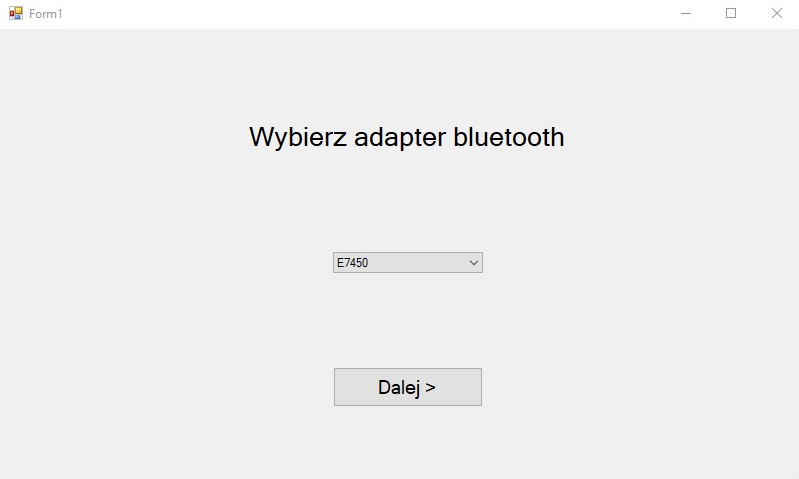
\includegraphics[scale=0.7]{ChooseAdapter}
\begin{lstlisting}
using [...]

namespace UP_Bluetooth
{
    public partial class ChooseAdapter : Form
    {
        private BluetoothRadio[] _adapters;

        public ChooseAdapter()
        {
            InitializeComponent();
        }

        private void Form1_Load(object sender, EventArgs e)
        {
            //Wyszukiwanie adapterow Bluetooth
            _adapters = BluetoothRadio.AllRadios;
            //Dodawanie nazw adapterow do Combo Boxa
            foreach (var adapter in _adapters)
            {
                comboBox1.Items.Add(adapter.Name);
            }

            comboBox1.SelectedIndex = 0;
        }

        private void button1_Click(object sender, EventArgs e)
        {
            //Wywolanie okna ChooseDevice
            BeginInvoke(new Action(() =>
            {
                using (var chooseDevice = new ChooseDevice(_adapters[comboBox1. SelectedIndex]))
                {
                    chooseDevice.ShowDialog();
                }
            }));
        }
    }
}

\end{lstlisting}
\newpage
\subsection{Okno wyboru urządzenia i przesyłania plików}

\noindent 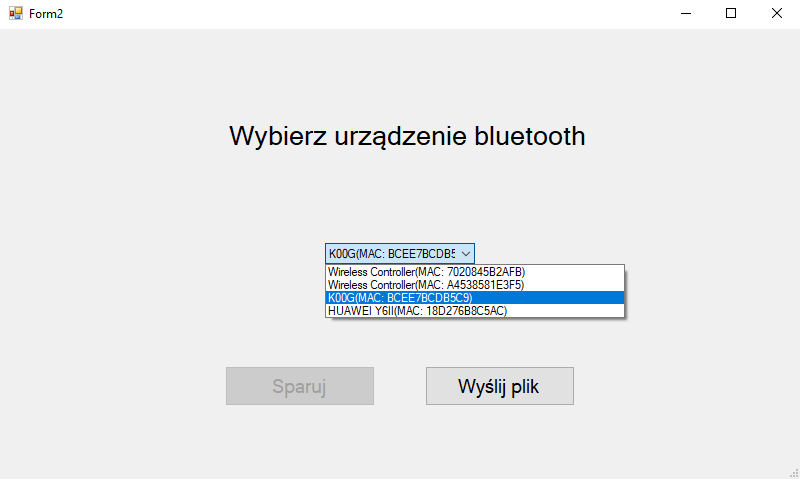
\includegraphics[scale=0.7]{ChooseDevice}
\begin{lstlisting}
using [...]

namespace UP_Bluetooth
{
    public partial class ChooseDevice : Form
    {
        private readonly BluetoothClient _client = new BluetoothClient();
        private BluetoothDeviceInfo[] _devices;
        private BluetoothDeviceInfo _chosenDevice;
        private readonly Thread _listener = new Thread(Listener);

        private static void Listener()
        {
            //Metoda nasluchujaca czy sparowane urzadzenia Bluetooth chca wyslac plik
            while (true)
            {
                //Stworzenie i uruchomienie sluchacza dla Bluetooth
                var listener = new ObexListener(ObexTransport.Bluetooth);
                listener.Start();
                //GetContext zwraca wartosc null jesli nie wykrywa zapytania od urzadzenia
                var obexContext = listener.GetContext();
                if (obexContext != null)
                {
                    var confirmResult = MessageBox.Show("Urzadzenie bluetooth chce wyslac plik. Czy chcesz go odebrac?",
                        "Przychodzacy plik",
                        MessageBoxButtons.YesNo);
                    if (confirmResult == DialogResult.Yes)
                    {
                        //Pobranie przychodzacego requesta z urzadzenia
                        var obexRequest = obexContext.Request;
                        //Ustalenie sciezki zapisu pliku na komputerze
                        var pathSplits = obexRequest.RawUrl.Split('/');
                        var fileName = @"C:\Users\DELL\Desktop\Politechnika\ " + "Semestr 5\Urzadzenia peryferyjne\LAB\UP_Bluetooth\ " + pathSplits[pathSplits.Length - 1];
                        //Zapisanie pliku
                        obexRequest.WriteFile(fileName);
                    }
                }
                listener.Stop();
            }
        }

        public ChooseDevice(BluetoothRadio chosenAdapter)
        {
            _listener.Start();
            InitializeComponent();
        }
        private async void ChooseDevice_Shown(Object sender, EventArgs e)
        {
            //Ekran ladowania "Wyszukiwane Urzadzen..."
            await Task.Run(() =>
            {
                //Wyszukiwanie urzadzen Bluetooth
                _devices = _client.DiscoverDevices();
                //Dodanie nazw i adresow MAC urzadzen do Combo Boxa
                foreach (var device in _devices)
                {
                    comboBox1.Items.Add(device.DeviceName + "(MAC: " + device.DeviceAddress + ")");
                }

                comboBox1.SelectedIndex = 0;
            }).ContinueWith(task => BeginInvoke(new Action(() =>
            {
                label2.Visible = false;
                button2.Visible = true;
                button1.Visible = true;
                comboBox1.Visible = true;
                label1.Visible = true;
            })));
        }
        private void button1_Click(object sender, EventArgs e)
        {
            //Ustawienie wybranego urzadzenia
            _chosenDevice = _devices[comboBox1.SelectedIndex];
            //Wyslanie prosby o parowanie, jesli zakonczy sie powodzeniem to aktywujemy przycisk do wyslania pliku
            if (BluetoothSecurity.PairRequest(_chosenDevice. DeviceAddress, "0000"))
            {
                button2.Enabled = true;
                button1.Enabled = false;
            }
            else
            {
                MessageBox.Show("Wystapil blad w trakcie operacji parowania", "Blad autoryzacji",
                    MessageBoxButtons.OK, MessageBoxIcon.Error);
            }
        }
        private void button2_Click(object sender, EventArgs e)
        {
            //Wysylanie pliku z komuptera do urzadzenia

            //Wybor pliku
            var result = openFileDialog1.ShowDialog();
            if (result == DialogResult.OK)
            {
                //Zapamietanie nazwy pliku
                var file = openFileDialog1.FileName;
                try
                {
                    _chosenDevice.Update();
                    _chosenDevice.Refresh();
                    //Umozliwienie wysylania plikow miedzy urzadzeniami
                    _chosenDevice.SetServiceState (BluetoothService.ObexObjectPush, true);
                    //Ustalenie sciezki pliku
                    var filePath = file.Replace(@"\\", @"\ ");
                    var fileToSend = new Uri("obex://" + _chosenDevice.DeviceAddress + "/" + filePath);
                    //Stworzenie requesta do wyslania pliku
                    var obexRequest = new ObexWebRequest(fileToSend);
                    //Wyslanie pliku
                    obexRequest.ReadFile(filePath);
                    //Zebranie informacji zwrotnej
                    var obexResponse = (ObexWebResponse)obexRequest. GetResponse();
                    MessageBox.Show(obexResponse. StatusCode.ToString());
                    obexResponse.Close();
                }
                catch (IOException)
                {
                }
            }
        }
        private void comboBox1_SelectedIndexChanged(object sender, EventArgs e)
        {
            //W zaleznosci od tego czy urzadzenia sa sparowane aktywujemy odpowiednie przyciski
            if (!_devices[comboBox1.SelectedIndex]. Authenticated)
            {
                button1.Enabled = true;
                button2.Enabled = false;
            }
            else
            {
                button1.Enabled = false;
                button2.Enabled = true;
            }
        }
    }
}


\end{lstlisting}
\end{adjustwidth}
\section{Wnioski}
Rozszerzenie 32feet.NET okazało się bardzo pomocne w wykonaniu ćwiczenia. Metody zawarte w nim znacząco ułatwiły wyszukiwanie adapterów i urządzeń Bluetooth, parowanie urządzeń i przesyłanie plików między nimi.
\end{document}